\documentclass[a4paper,12pt]{report}
 
\usepackage[utf8x]{inputenc} 
\usepackage[spanish]{babel}
 
\usepackage{hyperref}
\usepackage{amsmath}
\usepackage{titling}
\usepackage{microtype}
\usepackage{graphicx}
\usepackage{wrapfig}
\usepackage{enumitem}
\usepackage{fancyhdr}
\usepackage[scaled=.92]{helvet}
\usepackage{caption}
 
\captionsetup[figure]{font=small}
 
\setlength{\parskip}{1em}
 
\begin{document}
 
\let\cleardoublepage\clearpage
 
\title{\Large{\textbf{Modelos de animación}}}
\author{Heider Delgado 24981800}
\date{14 Marzo 2020}
 
\maketitle
 
\pagenumbering{gobble}
\tableofcontents
 

\thispagestyle{empty}
 
 
\renewcommand{\headrulewidth}{2pt}
\renewcommand{\footrulewidth}{1pt}

\newpage
\pagenumbering{arabic}
\chapter*{Introducción}
\addcontentsline{toc}{chapter}{Introduction} \markboth{INTRODUCTION}{}
 
Antes de hablar de modelos de animación, seria bueno definir los conceptos. 
Primero que son modelos: 
 
Los modelos son un arquetipo o punto de referencia para imitarlo
o reproducirlo
\cite{modelo}.
En computación gráfica de manera más general se refiere
a modelos dimensionales geométricos compuestos por vértices
,aristas y caras. 
Muchos modelos tienen índices los cuales se usan para determinar 
la conectividad de los vértices. 
La idea de tener un modelo es poder representar
objetos de forma que una computadora pueda entenderlo y mostrarlo.
 
 
Animación: La animación es un proceso utilizado por uno o
más animadores para dar la sensación de movimiento
a imágenes, dibujos u otro tipo de objetos inanimados 
(figuras de plastilina, por ejemplo). 
Se considera normalmente una ilusión óptica.\cite{animacion}
 
Entonces queda como definición de modelos de animación: 
Es tener un objeto geométrico y simular que se está moviendo.
 
 
\setcounter{page}{1}
\newpage
 
\chapter{Historia de la animación}
 
Desde tiempos ancestrales cuando el hombre descubrió su sombra en las fogatas de las cavernas
han surgido las primeras formas de animación estas luego fueron llamadas ``sombras chinescas''
estas referidas a solo los gestos de las manos o el cuerpo, 
que luego evolucionaron a objetos más elaborados y llegando así el ``teatro de las sombras'' que son
definidas como una proyección sobre una pantalla iluminada de sombras producidas por siluetas recortadas y manejadas mediante bastoncillos, aún no hilos como los de las
auténticas marionetas, que crean la ilusión de personajes entre los que tiene lugar una acción dramática.\cite{sombras_chinescas}
 
 
\begin{figure}[ht]
\centering
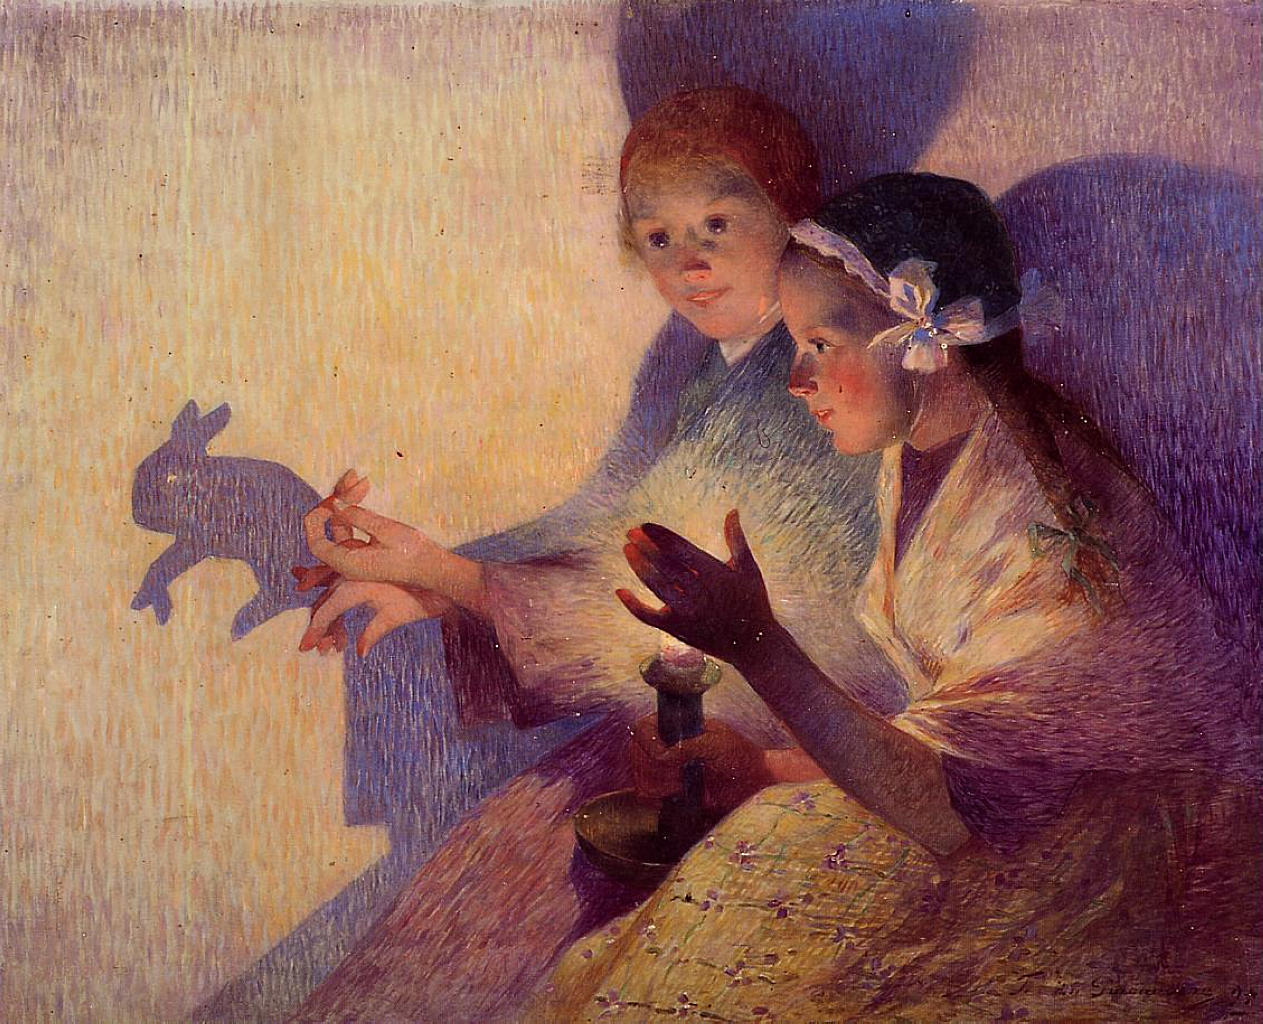
\includegraphics[height=6cm]{Imagenes/Puigaudeau}
\caption{El conejo (sombras chinescas), óleo de Ferdinand du Puigaudeau (1864-1930).}
\label{fig:sombras_chinescas_fig}
\end{figure}
 
 
\begin{figure}[!ht]
\centering
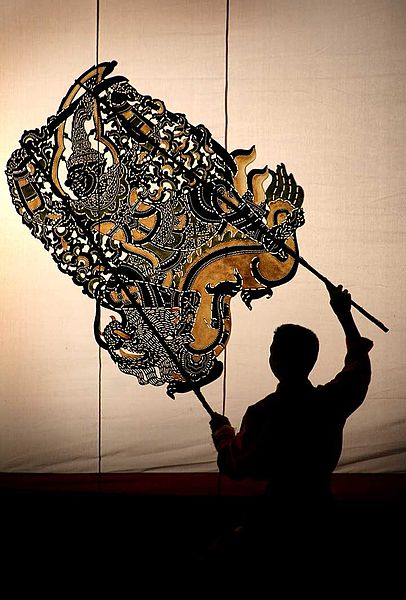
\includegraphics[height=6cm]{Imagenes/Nang_Yai_puppet}
\caption{Tradición de títeres «Nang Yai», en Camboya y Tailandia}
\label{fig:Nang_Yai_puppet}
\end{figure}
 
\newpage
 
Después de recorrer varios siglos llegamos al praxinoscopio: El praxinoscopio fue inventado por Charles-Emile
Reynaud, en 1876. Fue su primer invento.
Esta invención fue patentada en
1877, y obtiene una ``mención
honorable'' en la Exposición
Universal de París en 1878.
El praxinoscopio está compuesto
por una tira impresa removible
de una serie de 12 o 18 dibujos
colocados en un movimiento
cíclico, los espejos están dispuestos enfrente de las
imágenes. Cuando la cámara está funcionando, las imágenes
reflejado en los espejos comienzan a moverse y
dar a luz a un cortometraje.\cite{praxinoscope}
 
 
\begin{figure}[ht]
\centering
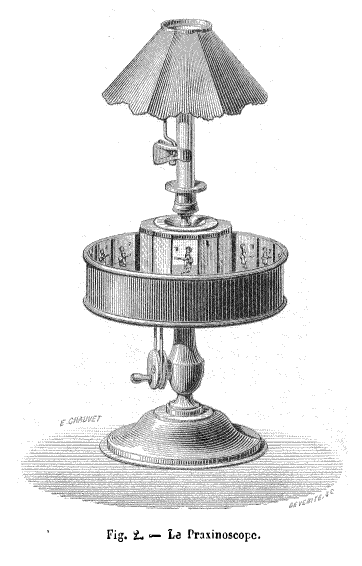
\includegraphics[height=6cm]{Imagenes/praxinoscope}
\caption{Ilustración del praxinoscopio de 1879}
\label{fig:praxinoscopio_ilus}
\end{figure}
 
 
\chapter{Historia de modelos de animación en computación}
 
La animación y los modelos de animación hechos en computadora divergen en su historia,
por eso se habló primero de cómo empezó la animación pero a mediados del siglo XX y después
de la segunda guerra mundial se empiezan a apreciar los primeros inventos para crear modelos de animación
por computadora.
 
 
\begin{figure}[ht]
\centering
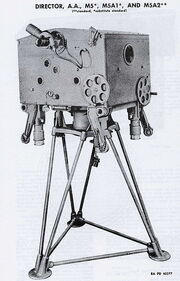
\includegraphics[height=6cm]{Imagenes/m5_director}
\caption{Versión de 1944 del director de armas M5, la versión de los Estados Unidos del Predictor Kerrison}
\label{fig:m5_director}
\end{figure}
 
 
\newpage
 
\section{Hitchcock’s Vertigo (1958)}
Hitchcock contrató a John Whitney para que hiciera una secuencia de apertura animada por computadora, Whitney 
instaló una computadora antiaérea de 850 libras 
y 11,000 componentes de la Segunda Guerra Mundial llamada 
\textit{M5 gun director} ver figura \ref{fig:m5_director} en una plataforma.
Era una computadora mecánica que necesitaba 
5 soldados para operar, pero no obstante, una computadora. 
Luego colocó celdas en una plataforma y usó un péndulo para lograr
la rotación sin fin necesaria. 
Colaboró con el diseñador gráfico Saul Bass. 
Esta se considero como la primera animación realizada por computadora de la historia.\cite{john_whitney} 
Whitney y las técnicas que desarrolló con esta máquina fueron 
lo que inspiró a Douglas Trumbull (asistente especial de efectos especiales) a utilizar la técnica de exploración de hendidura \textit{the slit scan technique} en la película
``2001: Una odisea del espacio'' (1968)
 
 
\begin{figure}[ht]
\centering
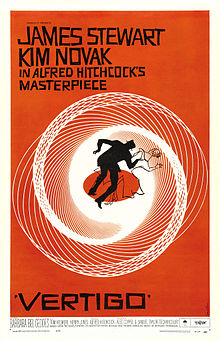
\includegraphics[height=6cm]{Imagenes/Vertigomovie}
\caption{Cartel de estreno teatral de Saul Bass}
\label{fig:vertigo}
\end{figure}
 
 
\section{Computer Sketchpad (1962)}
Ivan Sutherland presentó \textit{``Sketchpad''} en 1962 en su tesis: los puntos podrían marcarse en un monitor.
 
El sistema \textit{Sketchpad} utiliza el dibujo como un nuevo medio de comunicación para
un ordenador. El sistema contiene programas de entrada, salida y cálculo.
que le permiten interpretar información dibujada directamente en una pantalla de computadora.
Se ha utilizado para dibujar modelos eléctricos, mecánicos, científicos, matemáticos y
dibujos animados. Es un sistema de propósito general. Sketchpad ha mostrado ser
muy útil como ayuda para la comprensión de los procesos, como la noción de enlaces, que se puede describir con imágenes. Sketchpad también hace
fácil dibujar dibujos muy repetitivos o muy precisos y cambiar
dibujos previamente dibujados con ella.\cite{sketchpad}
 
\begin{figure}[ht]
    \centering
    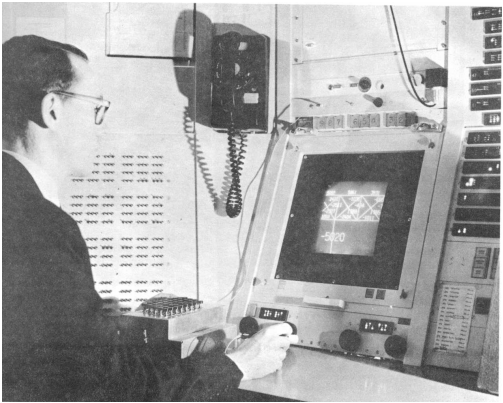
\includegraphics[height=6cm]{Imagenes/sketch}
    \caption{ÁREA OPERATIVA TX-2 - SKETCHPAD EN USO. En la pantalla
    se puede ver parte de un puente que sostiene el autor
    La pluma de luz. Los botones que se utilizan para controlar funciones de dibujo específicas se encuentran en el cuadro frente al autor. Parte del banco de interruptores se puede ver detrás del autor. 
    El tamaño y la posición de lo que se ve en la pantalla se obtiene a través de los cuatro botones negros justo encima de la mesa.}
    \label{fig:sketch_img}
\end{figure}
 
\section{Computer Animated Hand (1972)}
 
 
Dirigido por Ed Catmull (más tarde trabajaría en Pixar) y Fred Parke, el corto muestra una mano animada por computadora, así como rostros humanos.
La película fue incluida en el \textit{National Film Registry} en 2011.
 
Fred Parke, un compañero Ph.D. El estudiante de su clase que ayudó a producir la película, recordó que la animación por computadora estaba ``en el borde loco en ese momento. La gente apenas llegaba 
al punto en que podían obtener una computadora para sacar imágenes fijas''. \cite{animated_hand1}
 
 
\begin{figure}[ht]
    \centering
    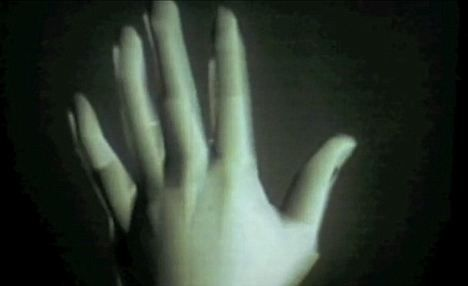
\includegraphics[height=6cm]{Imagenes/computer_animated_hand}
    \caption{Ed Catmull, cofundador de Pixar Animation Studios, 
    conocido por sus películas animadas CGI (imagen generada por computadora), 
    creó un programa para animar digitalmente una mano humana en 1972 
    como un proyecto de estudiante graduado}
    \label{fig:computer_animated_hand}
\end{figure}
 
 
Presenta una mano giratoria tridimensional renderizada en gráficos de computadora prístinos. 
Fue un proyecto de investigación científica pionero y
una visión del potencial técnico de la computadora como herramienta para la animación, 
A Computer Animated Hand coloca al frente y al centro el papel del ``arte'' de la construcción 
de imágenes digitales.\cite{animated_hand2}
 
 
\section{Adam Powers, The Juggler (1981)}
 
Se mostraba el potencial narrativo que podría tener los modelos de animación.
 
Este cortometraje animado por computadora fue producido por 
Information International Inc. (III) como muestra de la exposición anual 
de la Asociación SIGGraph de la Asociación de Maquinaria de 
Computación en 1981. Al mostrar el potencial narrativo
de la innovadora técnica de modelado poligonal de CGI y III,
la película condujo directamente a la participación 
tanto de la compañía como del productor Richard F. Taylor 
en el innovador largometraje de Disney Tron.\cite{the_juggler}
 
\newpage
 
\begin{figure}[ht]
    \centering
    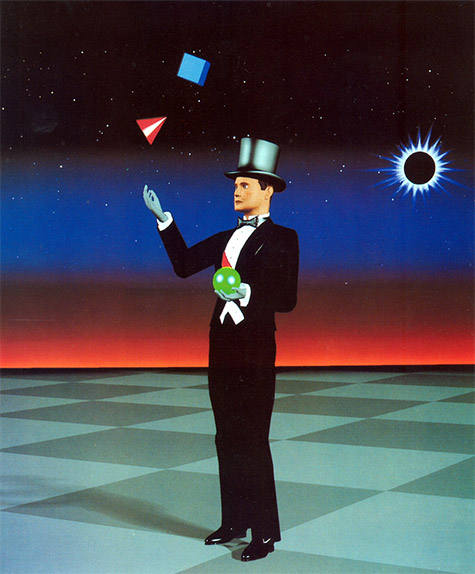
\includegraphics[height=6cm]{Imagenes/adam_powers_the_juggler}
    \caption{Adam Powers, the juggler: arte del póster de presentación en SIGGRAPH 1991}
    \label{fig:adam_powers_the_juggler}
\end{figure}
 
 
El \textit{ASAS (Actor/Scriptor Animation System)} frecuentemente juega un papel
central en la animación comercial y producción en III, aunque otras técnicas de animación
utilizan controles. Los proyectos realizados con ASAS incluyen, el logotipo animado ``MICROMA'',
el logotipo animado de "LBS", noticias de TV "NEWS CENTER 2"
Introducción al show, dos comerciales de TV para ``TORNADO'', varios
anuncios de revistas, toda la animación del tema para la Muestra III 1981
Reel (``The Juggler''), aproximadamente la mitad de los efectos especiales para la película Ladd
característica de la compañía ``LOOKER'', y todos los
animación e imágenes fijas III está haciendo para el recientemente lanzado
Característica de Disney ``TRON''.\cite{asas_tron}
 
 
\begin{figure}[ht]
    \centering
    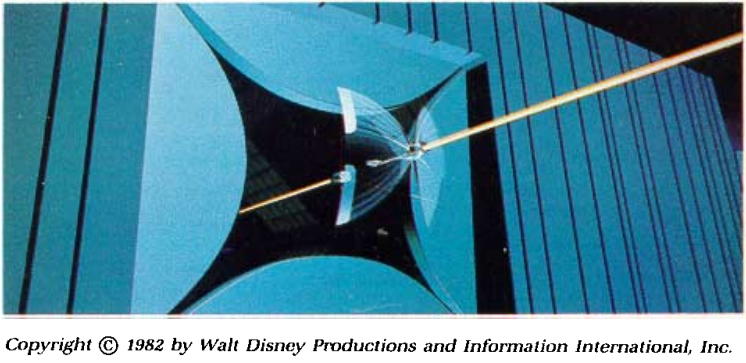
\includegraphics[height=6cm]{Imagenes/tron}
    \caption{Secuencias Solar Sailer Escape de TRON}
    \label{fig:tron}
\end{figure}
 
 
 
\section{Immersion (1994)}
 
Los métodos de modelado y representación basados en imágenes 
(IBMR en ingles \textit{Image-based modeling and rendering}) se basan en un conjunto de imágenes bidimensionales 
de una escena para generar un modelo tridimensional 
y luego generar algunas vistas novedosas de esta escena.
 
 
El modelado y la representación basados en imágenes (IBMR) pueden abordar ambas
cuestiones. Con IBMR, tanto la estructura como la apariencia de la escena se derivan de
fotografías del mundo real, que no solo pueden simplificar la tarea de modelado, sino también cuando son
empleados juiciosamente puede reproducir el realismo presente en las fotografías del mundo real. \cite{IBMR}
 

Los estudios de dimensionalización comenzaron como una colaboración informal entre los investigadores de la visión por computadora y otros de nosotros
construyendo el equipo de cámara estereoscópica para \textit{See Banff Kinetoscope project}, en \textit{Interval Research} en 1993. Los investigadores de la visión por computadora ayudaron con las
especificaciones para la cámara, lo que resultó en imágenes utilizables para su trabajo y para el nuestro. 
Los estudios aquí se basan en derivar información de profundidad de pares de imágenes estereoscópicas,
luego convierte los píxeles 2D en "puntos en el espacio" 3D.\cite{immersion}
 

\newpage
 
\begin{figure}[!ht]
    \centering
    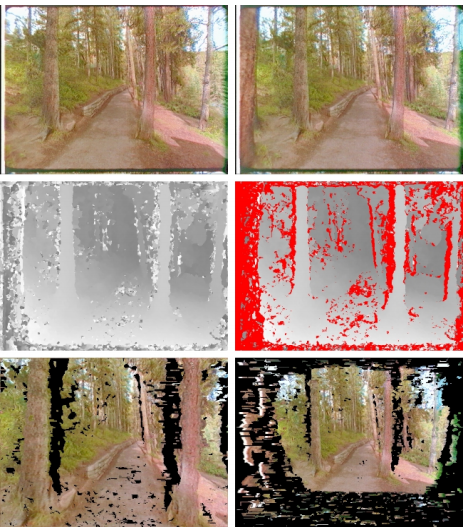
\includegraphics[height=10cm]{Imagenes/immersion_img}
    \caption{Las dos imágenes del tope son
    un par estéreo (invertido para la visualización estéreo cruzada) tomada en el Bosque Nacional de Banff. 
    En la mitad la foto de la izquierda es un mapa de disparidad estéreo producido por la implementación paralela de John Woodfill del
    Algoritmo estéreo Zabih-Woodfill \cite{Zabih_Woodfill} A su derecha, el mapa se ha procesado 
    con un comando de verificación de consistencia de izquierda a derecha para invalidar regiones 
    donde se ejecuta estéreo basado en la imagen izquierda y estéreo
    basado en la imagen correcta, esto no produjo resultados consistentes.
    Las ultimas dos imagenes se muestran dos vistas virtuales generadas
    lanzando cada píxel al espacio calculada en función de su estimación de profundidad y reproyectando los
    píxeles en nuevas posiciones de cámara. A la izquierda está el resultado de moverse virtualmente 
    un metro hacia adelante, a la derecha es el resultado de prácticamente moverse un metro hacia atrás. 
    Tenga en cuenta las áreas oscuras desoladas son producidas por estos movimientos de cámara virtual; 
    Estas áreas no se vieron en el par estéreo original. En
    las animaciones de Inmersión '94 (disponibles en http://www.debevec.org/Immersion, estas regiones
    se rellenaron automáticamente desde pares estéreo vecinos.}
    \label{fig:immersion_img}
\end{figure}
 
 
\newpage
 
 
\section{Toy Story (1995)}
 
 
Toy Story, la primera función animada generada por computadora de longitud completa
la película (lanzada en 1995) se estableció como un visual
punto de referencia para las computadoras tanto como en hardware de gráficos y desarrollo de software.
Poco después del debut de la película, los fabricantes de chips gráficos
quería saber cómo podían calcular las imágenes de la calidad Toy-Story en una PC; 
los desarrolladores de juegos querían saber cómo podrían ofrecer animaciones de calidad 
Toy-Story en consolas de juegos; e investigadores en robótica quería saber cómo podían construir inteligencia artificial
en sus máquinas para lograr personajes realistas de la calidad Toy-Story.
 
 
Como supervisor de sombreado y efectos visuales enm Toy Story original, Tom Porter dirigió un grupo de artistas técnicos 
que trabajaban en todas las apariencias de la superficie de la película, junto con ciertos efectos visuales para que fuera la corriente principal del proceso de animación de personajes de Pixar.
 
 
En 1995, Pixar usaba un solo procesador de 150Mhz,
Máquinas SGI Indigo2 con 64Mb de memoria para cada animador y  director técnico, junto con
100 Sun Microsystems Sparc 20 de doble procesador
máquinas en la empresa ``renderfarm''. La representación final incluyó 77 
minutos de imágenes, o la totalidad
duración de la película. (El renderizado fue de 24 fotogramas por
segundo a 1536x922 píxeles de resolución.)\cite{toy_story}
 
 
\begin{figure}[bt]
    \centering
    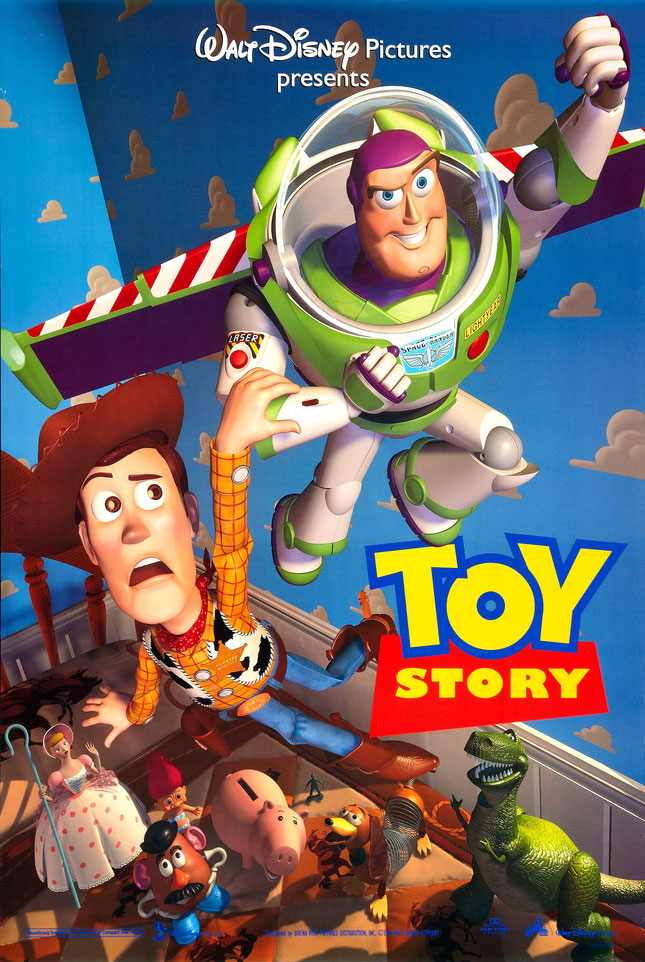
\includegraphics[height=10cm]{Imagenes/toy story}
    \caption{Toy Story poster}
    \label{fig:toy_story_poster}
\end{figure}
 
 
\begin{figure}[ht]
    \centering
    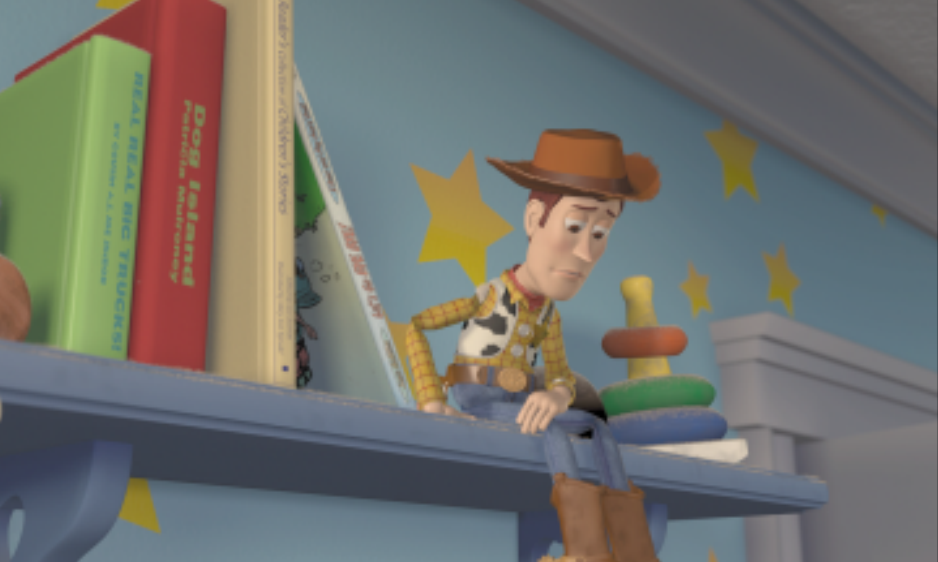
\includegraphics[height=6cm]{Imagenes/woody_sitting}
    \caption{Woody is shelved in Toy Story 2}
    \label{fig:woody_sitting}
\end{figure}
 
 
\chapter{Principios de la animación}
 
 
\textit{``When we consider a new project, we really study it ... not just the surface idea,
but everything about it''}
 
\hspace*{\fill}{\rm --- Walt Disney}
 
 
\hspace*{\fill}
 
 
Los animadores seguian buscando mejores métodos de relacionar dibujos con 
otros y encontraron pocas maneras de producir resultados predecibles.
No podian esperar exito todo el tiempo, pero estas técnicas especiales de dibujar un personaje en movimiento
ofrecían cierta seguridad. Mientras cada uno de estos procesos adquiria un nombre, se fue hablando de ello, 
analizando y perfeccionando, y cuando un nuevo artista era contratado
se le enseñaba estas prácticas como si fueran reglas del arte.
Para la sorpresa de todos, estas reglas se convirtieron en los 
principios principales de la animación:\cite{principles_animation}
 
 
\section{Aplastar y estirar \textit{(Squash and Stretch)}}
 
Por lejos el mayor de los descubrimientos es lo que llamamos
\textit{Squash and Stretch}. Cuando una figura es movida en el papel de un dibujo al siguiente,
hay una rigidez marcada que es enfatizada por el movimiento. En la vida real esto solo ocurre con los objetos más rígidos,
como sillas, platos y sartenes. Pero cualquier cosa que esté viva, sin importar cuantos huesos tiene, 
enseñará un cambio considerable en su forma mientras realiza acciones.\cite{principles_animation}
 
 
\begin{figure}[ht]
    \centering
    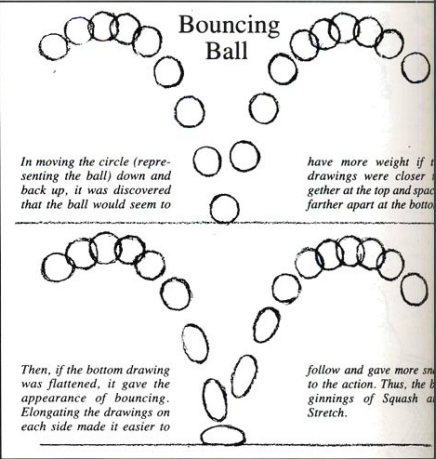
\includegraphics[height=6cm]{Imagenes/bouncing_ball}
    \caption{Un círculo en movimiento (representado una pelota) cayendo y rebotando, se descubrió que la pelota paraceria
    tener más peso si más dibujos estuvieran más cercanos en el tope y más alejados en el piso. Después, si el dibujo que tocara el suelo estuviera aplanado
    da la apariencia de rebote. Alargando los dibujos de lado y lado parecia mas facil de seguir y cercano a la acción. Estos fueron los comienzos de
    Aplastar y Estirar (\textit{Squash and Stretch})}
    \label{fig:bouncy_ball}
\end{figure}
 
 
\section{Anticipacion (\textit{Anticipation}) }
 
 
Para las personas en la audiencia viendo una escena animada no podrían entender los eventos en la pantalla
a menos de que haya una secuencia planeada de las acciones que los guíe de manera clara a la siguiente actividad.
La audiencia debe estar preparada para el próximo movimiento y esperarlo antes de que ocurra. Esto se logra
precediendo cada acción importante con un movimiento especifico que anticipa a la audiencia
de qué es lo que va a suceder. Esta anticipación puede ser tan pequeño como un cambio en la expresión
o tan grande como la mayor de las acciones físicas. Antes de que una persona corra, se agacha, encogiéndose como un resorte,
o, al contrario, se abalanza en la dirección opuesta, levantando sus brazos y hombros y una pierna, mientras mira el lugar
de su próxima acción.\cite{principles_animation} 
 
 
\begin{figure}[!ht]
    \centering
    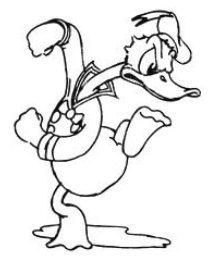
\includegraphics[height=6cm]{Imagenes/donald_anticipation}
    \caption{Se abalanza hacia la izquierda con la anticipación de su proximo movimiento}
    \label{fig:donald_anticipation}
\end{figure}
 
\newpage
 
\section{Puesta en escena (\textit{Staging})}
 
\textit{``Staging''} es uno de los principios más generales porque encapsula muchas áreas y se remonta al teatro.
Su significado, sin embargo, es muy preciso: es la presentación de una idea de tal forma que sea completamente
y sin lugar a dudas clara. Una acción es puesta en escena para que sea entendida, una personalidad que sea reconocida de manera sencilla,
una expresión que pueda ser vista, un estado de ánimo que afecte a la audiencia. Se maximiza la comunicación de esto
cuando la puesta en escena es correctamente preparada.\cite{principles_animation}
 
 
Se hacen los dibujos de manera que invoquen la idea de la mejor y más simple manera antes de saltar a la siguiente acción.
Se está diciendo en efecto ``Mira a esto---ahora mira a esto---ahora mira a esto.'' Se asegura de que la camara este a la distancia correcta del personaje
para mostrar que está haciendo. Si está pateando, no se necesita la camisa mostrando su cintura. Si estás mostrando una expresión
no lo haces en una toma lejana donde la figura se pierde con el fondo.\cite{principles_animation}
 
 
\begin{figure}[ht]
    \hspace*{-2cm}
    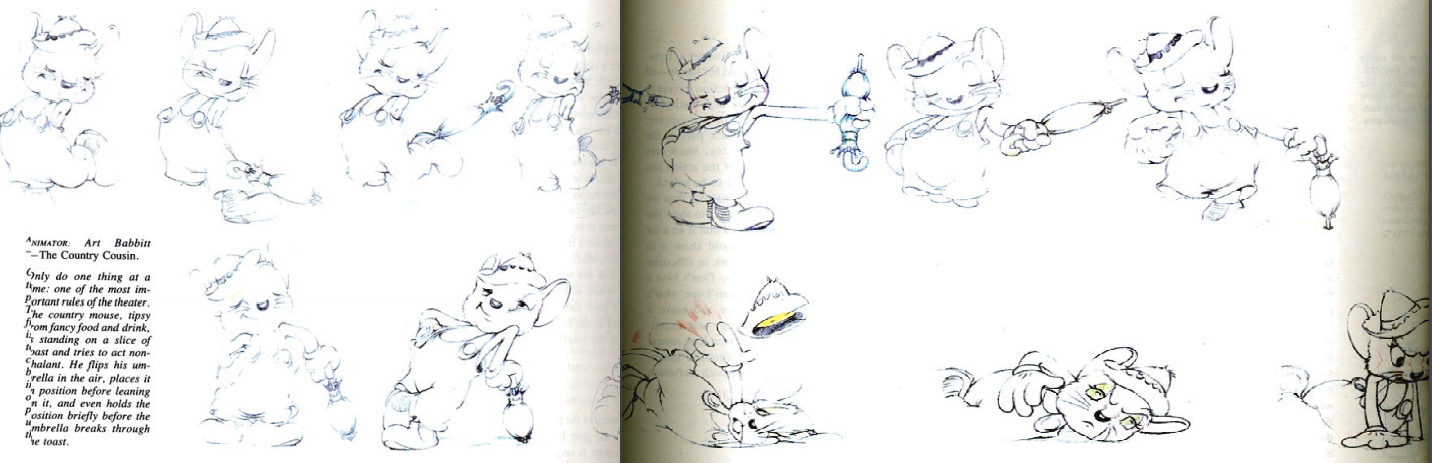
\includegraphics[height=6cm]{Imagenes/the_country_cousin}
    \caption{Animador: Art Babbitt ---The Country Cousin.
    Solo una cosa a la vez: una de las reglas más importantes del teatro. El ratón de campo, achispado de bebidas y comidas lujosas,
    mientras está parado sobre una pieza de pan tostado trata de actuar despreocupado. Le da vueltas a su paraguas en el aire, lo coloca en posición
    para luego recostarse en él, y mientras mantiene la posición por un breve momento antes de que el paraguas rompa a través del pan}
    \label{fig:the_country_cousin}
\end{figure}
 
 
\section{Animación directa y pose a pose (\textit{Straight Ahead Action and Pose to Pose)}}
 
 
Hay dos maneras de desarrollar una animación. La primera conocida como animación directa (\textit{Straight Ahead Action)}
porque el animador literalmente trabaja hacia adelante desde su primer dibujo en la escena. Sencillamente empieza haciendo un
dibujo y luego el siguiente, tomando las ideas mientras dibuja, hasta que llega al final de la escena. El animador sabe los puntos
narrativos de la escena y lo que debe ser incluido. Pero no tiene un plan trazado como todo será hecho al momento de iniciar.
Ambos dibujos y acciones tienen una apariencia fresca y estrafalaria, mientras el animador mantiene todo el proceso de manera creativa.\cite{principles_animation}
 
 
La segunda forma es llamada pose a pose (\textit{Pose to Pose.}) En este caso, el animador planea sus acciones, resolviendo qué acciones necesitas ser elaboradas para animar la historia, hace los dibujos, relacionando cada uno con su tamaño y acción,
y da a la escena a su asistente para dibujar los intermedios. Cada escena es siempre fácil de seguir y se trabaja bien porque la relaciones han sido
cuidadosamente consideradas antes de que el animador se adentre mucho en los dibujos. Se emplea más tiempo en mejorar dibujos importantes y en ejercitar
mayor control sobre el movimiento. Con Pose a Pose, hay claridad y fuerza. Con Animación directa, hay espontaneidad.\cite{principles_animation}
 
 
\begin{figure}[ht]
    \hspace*{-1cm}
    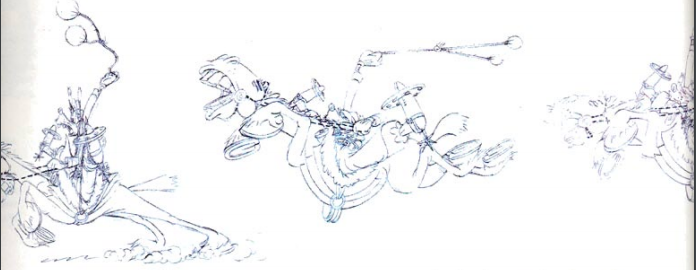
\includegraphics[height=6cm]{Imagenes/el_guacho_goofy}
    \caption{Animador: Woolie Reitherman ---El Guacho Goofy.
    Ejemplo de animación \textit{``Straight Ahead.''} El animador normalmente se sorprende como cualquiera
    de la manera en que la escena termina.}
    \label{fig:el_guacho_goofy}
\end{figure}
 
 
Los dos métodos aún están en uso porque los dos ofrecen ciertas ventajas para los diferentes tipos de acción.
 
 
\section{Acciones complementarias y superpuestas \textit{(``Follow Through and Overlapping Action'')}}
 
 
Cuando un personaje que entra en escena y a alcanzado un punto para la siguiente acción,
muy seguido entraba súbitamente a un estado completo de alto.
Esto era rígido y no se veía natural, pero nadie sabia que hacer al respecto.
Walt estaba preocupado. ``Las cosas no se detienen completamente de una sola vez,
chicos; primero una parte y luego otra.''
Varias maneras diferentes fueron eventualmente encontradas para corregir estas condiciones;
Eran llamadas
\textit{(``Follow Through'')} o \textit{(``Overlapping Action''} y nadie sabía cuando
una terminaba y la otra empezaba.
Al parecer habia cinco categorias:
 
 
\begin{enumerate}
    \item Si el personaje tiene algún accesorio, como orejas largas o una cola o un abrigo enorme, estas partes continuaban moviéndose luego de que el resto de la figura se detenía.
    \item El cuerpo en si no se mueve todo de una sola vez, pero al contrario se estira, se recupera, se tuerce, se da vuelta, y contrae mientras la forma trata de trabajar uno contra otro. Mientras una parte llega al punto de detenerse, otras partes pueden estar todavía en movimiento; un brazo o una mano pueden continuar su acción luego de que el cuerpo está en su pose final.
    \item Partes flojas de la piel de una figura, como las mejillas, o algunas partes del cuerpo, se moverían a una tiempo más lento que otras partes del esqueleto, este barrido hacia atrás de las acciones es llamado comúnmente como arrastre \textit{``drag''} y da flexibilidad y solidez a la figura que es fundamental para dar el sentimiento de que está vivo. Cuando se realiza correctamente, esta técnica es casi indetectable mientras la película está siendo proyectada.
    
 
    \begin{figure}[ht]
        \centering
        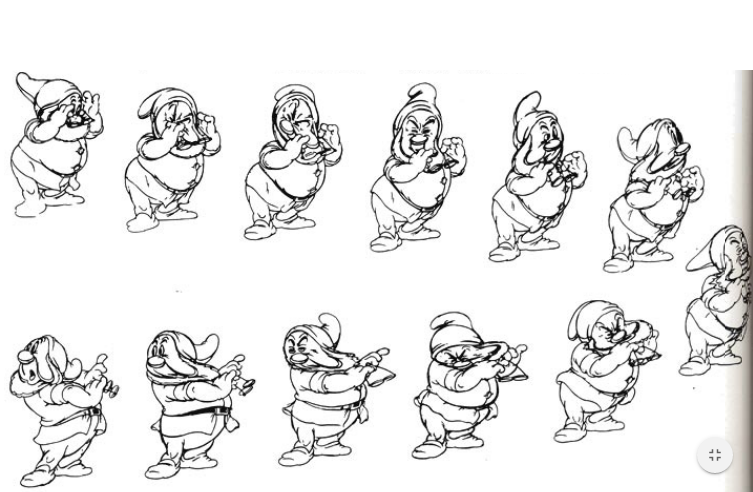
\includegraphics[height=6cm]{Imagenes/enano_sabio}
        \caption{Enano sabio mientras se quita los lentes y gira su cabeza, ejemplo de \textit{(``Follow Through and Overlapping Action'')}}
        \label{fig:enano_sabio}
    \end{figure}
 
 
    \item La manera en que una acción es terminada la mayoria de las veces nos dice más sobre el personaje que los dibujos del movimiento en sí. Un golfista realiza un poderoso swing, que cubre solo unos pocos paneles, pero lo que sucede con el luego puede tomar fácilmente cinco metros de película y es más revelador.
    \item Finalmente, está el movimiento en el lugar \textit{``Moving hold''}, por el cual emplea partes de todos los elementos de Acciones complementarias y superpuestas \textit{(``Follow Through and Overlapping Action'')} para alcanzar un nuevo sentimiento de vida y claridad.\cite{principles_animation}
 
 
    \begin{figure}[ht]
        \hspace*{-2cm}
        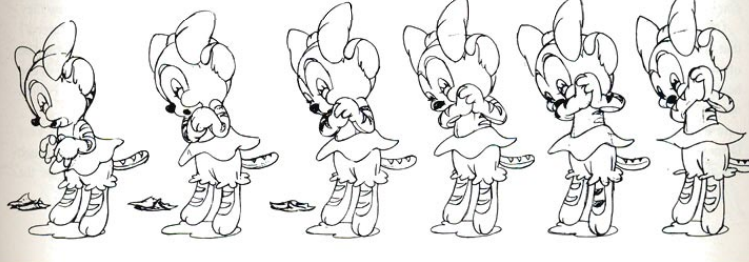
\includegraphics[height=6cm]{Imagenes/moving_hold}
        \caption{``Primero esta pose, luego te deslizas a otra poze mas fuerte---todo aumentado al máximo, las mejillas suben, las orejas vuelan hacia arriba, las manos se elevan, se pone en puntillas, sus ojos se abren más, pero esencialmente
        sigue en pose''}
        \label{fig:moving_hold}
    \end{figure}
 
\end{enumerate}
 
 
\section{Acelerar y desacelerar \textit{``Slow in and slow out''}}
 
 
Una vez el animador a trabajado sobre sus poses (los ``extremos'') y
redibujado hasta que sus dibujos fueran los mejor que él podía hacer,
él naturalmente quería que la audiencia lo viera.
El sincronizaba los dibujos fundamentales para que se movieran rápido de uno a otro,
para que gran parte de las imágenes de la escena estuvieran en o cerca de estos ``extremos.''
Poniendo varios intermedios cerca de cada extremo y solo pocas imágenes en la mitad de
la cinta, el animador lograba un resultado enérgico con los
personajes cambiando de una actitud a la otra. 
Esto se llamó \textit{``Slow in and slow out''}, 
puesto que esta era la manera en que los intermedios eran sincronizados.
Si se utilizaba mucho de esta técnica daba el sentimiento de una acción mecánica,
robando a la escena de la esencia de vida que buscaba, 
pero aun asi se convirtio en un importante descubrimiento que luego se convertiría en la base
de refinamiento entre la sincronización
(\textit{``Timing''}) y la puesta en escena (\textit{Staging}).\cite{principles_animation}
 
 
\section{Arcos \textit{``Arcs''}}
 
 
Muy pocos organismos son capaces de hacer movimientos que parezcan mecánicos o con precisiones de arriba a abajo.
La acciones de un pájaro carpintero podría ser la excepción, y, por las restricciones de un cuerpo esquelético externo, hay muchos ejemplos en el mundos de los insectos, pero los movimientos de la
mayoría de los seres vivos siguen un camino ligeramente circular. La cabeza raramente se empuja hacia afuera y luego hacia adentro; sube ligeramente, o baja cuando regresa.
Tal vez esto tenga que ver con el peso o tal vez con la estructura interna de las formas de vida mas complejas, pero, por cualquier razon, la mayoria de los movimientos describirán arcos de alguna u otra forma.\cite{principles_animation}
 

\begin{figure}[ht]
    \centering
    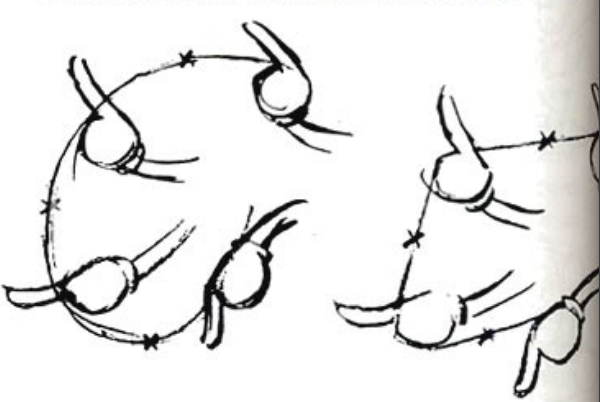
\includegraphics[height=6cm]{Imagenes/circular_hand}
    \caption{La acción de un dedo apuntado con la mano sigue un camino circular. El animador mapea
    las posiciones de sus dibujos en este arco. Realizando sus dibujos clave, indicando donde los intermedios deberían estar para
    seguir la acción de este arco. Los intermedios que no siguen este arco cambian la acción radicalmente.}
    \label{fig:circular_hand}
\end{figure}
 

Este descubrimiento hizo un cambio mayor en la forma en que los animadores diseñan movimientos a sus personajes,
rompiendo con la rigidez y dureza de como se realizaban las acciones antes.\cite{principles_animation}
 
 
\section{Acción secundaria \textit{``Secondary Action''}}
 
 
A menudo, la idea de de ser puesto en escena puede ser fortalecida por acciones subsidiarias del cuerpo. 
Una figura triste se limpia las lágrimas mientras voltea. 
Alguien en aturdido menea su cabeza mientras se levanta. 
Una persona nerviosa se pone los lentes mientras recobra la calma. 
Cuando estas acciones apoyan la acción principal se llaman acciones secundarias \textit{``Secondary Action''} 
y siempre es subordinada a la acción principal. Si hace conflicto o se vuelve más interesante o dominante a la acción principal,
entonces o es una mala elección o no se puso en escena correctamente.\cite{principles_animation}
 
\begin{figure}[ht]
    \centering
    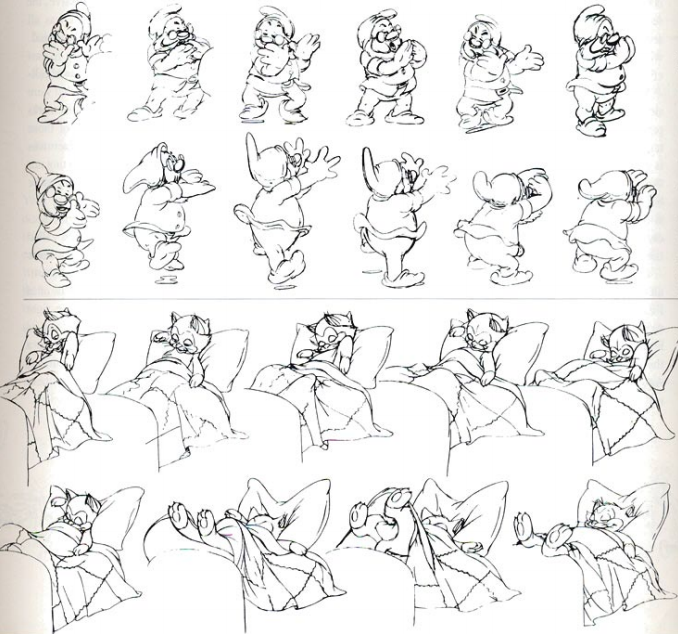
\includegraphics[height=12cm]{Imagenes/secundary_action}
    \caption{La dificultad principal se encuentra en tratar de unificar el dibujo
    y la sincronización como separados pero relacionados. Un animador encontró que la mejor manera era a través de ``building block'', primero animaba las acciones importante y luego repasaba la escena y animaba la acción secundaria.}
    \label{fig:secundary_action}
\end{figure}
 
 
Cuando son usadas correctamente, las acciones secundarias añaden riqueza a la escena, naturalidad a la acción y le dan dimensiones a la personalidad del personaje.
 
 
\section{Sincronización \textit{``Timing''}}
 
 
La cantidad de dibujos usados en un movimiento determina la cantidad de tiempo que esa acción tendrá en pantalla.
Si los trazos son simples, claros, y expresivos, la punto argumental puede terminar rápidamente, y esto era todo en lo que se preocupaban los animadores en sus inicios.
La sincronización (\textit{``Timing''}) en estos dibujos era limitada a movimientos rápidos o movimientos lentos, con acentos y golpes clamando por un manejo especial.\cite{principles_animation}
 
 
La complicada relación que vino con las acciones secundarias y las acciones complementarias hizo un llamado por refinamientos extensivos, pero aun los movimientos más básicos
mostraron la importancia de la sincronización (\textit{``Timing''}) y la constante necesidad de su estudio.
 
 
No intermedios: EL PERSONAJE ha sido golpeado por una fuerza increíble. Su cabeza casi sale despedida.
 
 
Un intermedio: ... ha sido golpeado por un ladrillo, un rodillo, o una sartén de freír.
 
 
Dos intermedios: ... tiene un tic nervioso, un espasmo muscular, una incontrolable contraccion.
 
 
Tres intermedios: ... está esquivando el ladrillo, rodillo, o sarten.
 
 
Cuatro intermedios: ... esta dando una orden nitida, ``¡Empieza a moverte!'' ``¡Muévete!''
 
 
Cinco intermedios: ... es más amigable ``Aquí.'' ``Vamos---¡Apurate!''
 
 
Seis intermedios: ... observa a una mujer atractiva, o el carro deportivo que siempre quiso.
 
 
Siete intermedios: ... trata de ver mejor algo.
 
 
Ocho intermedios: ... busca por la mantequilla de maní en el estante de la cocina.
 
 
Nueve intermedios: ... evalua, considera profundamente.
 
 
Diez intermedios: ... estira un dolor muscular.\cite{principles_animation}
 
 
\begin{figure}[ht]
    \centering
    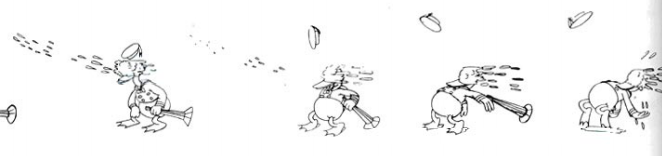
\includegraphics[height=3cm]{Imagenes/timming1}
    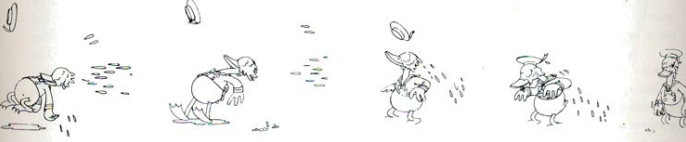
\includegraphics[height=3cm]{Imagenes/timming2}
    \caption{El pato Donald siendo golpeado por una bola de nieve.}
    \label{fig:timming1}
\end{figure}
 
 
 
\section{Exageración \textit{``Exaggeration''}}
 
 
Habia una confusión entre los animadores cuando Walt dijo la primera vez que queria más realismo y luego criticó el resultado porque no eran lo suficientemente exagerado.
En la mente de Walt, probablemente no había diferencia. El creia en en ir al corazón de todo y desarrollar la esencia de lo que había encontrado.
Si un personaje estaba triste, hazlo mas triste, alegre, mas alegre; preocupado, más preocupado; salvaje, más salvaje.
Algunos artistas han sentido la necesidad de ``exageración'' significaba dibujos mas distorsionados, o una acción tan violenta que fuera inquietante.
Encontraron que ese no era el punto.\cite{principles_animation}
 
 
Cuando Walt hablaba de realismo, el quería una caricaturarizacion del realismo. Un artista lo analizó correctamente cuando dijo,
``No creo que se refiera a `realismo.' Creo que se refiere a que algo sea más convincente, que hiciera un mejor contacto con las personas, y el solo
dijo `realismo' porque las cosas `reales' hacen ... Algunas veces [en la animación] el personaje haría algo inconveniente, orden
para enseñar hábil era el animador, y no era real, era falso'' Walt no aceptaba nada que destruyera la credibilidad. 
Pero el raramente le pedía a los animadores reprimir una acción a menos que fuera adecuado para la escena.\cite{principles_animation}
 
 
\begin{figure}[ht]
    \centering
    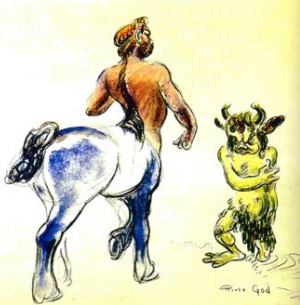
\includegraphics[height=6cm]{Imagenes/exageration}
    \caption{``Cuando estaba dirigiendo solía decirle a los animadores, `¿harías algo por mi? ¿Lo harías tan extremo como para que me moleste?' ''---Dave Hand}
    \label{fig:exageration}
\end{figure}
 
 
 
\section{Dibujo sólido \textit{``Solid Drawing''}}
 
 
Los de la vieja generación eran presionados para seguir las demandas del nuevo tipo de animación.
Más de una vez un mejor hombre aconsejaba a las principiantes, ``Deberías aprender a dibujar bien antes de empezar a animar.''---Grim Natwick.
 
Muchos anuncios eran colgados para asegurarse de que los jóvenes pasantes los vieran ``¿Tu dibujo tiene peso, volumen y balance?''---un recordatorio casual
de los fundamentos de los sólidos y los dibujos en tres dimensiones.\cite{principles_animation}
 
\begin{figure}[ht]
    \centering
    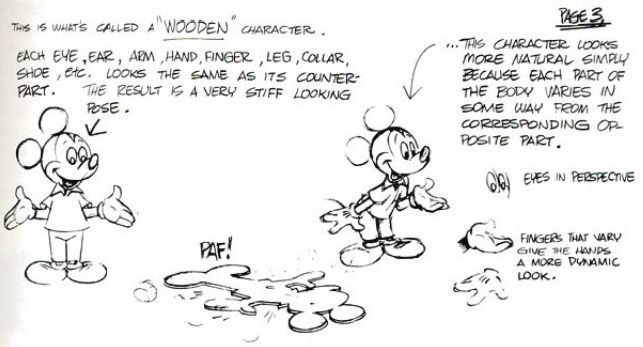
\includegraphics[height=6cm]{Imagenes/wooden_character}
    \caption{Instrucciones de como dibujar con profundidad.}
    \label{fig:wooden_character}
\end{figure}
 
 
El objetivo principal era hacer una figura ``animable'', que fuera capaz de tener volumen pero aun así ser flexible, que poseyera fuerza sin ser rígido, 
y que nos diera oportunidades para movimientos que se adaptaran a nuestras ideas. Necesitamos una figura que tuviera una forma viva, listo para moverse---en contraste
con una figura estática. Utilizaremos el término ``plástico'' y solo la definición de la palabra parecía transmitir el sentimiento de una actividad en el dibujo.
``Capaz de ser formado o reformado, flexible.''\cite{principles_animation}
 
 
\section{Atractivo \textit{``Appeal''}}
 
 
El atractivo \textit{``Appeal''} era muy importante desde el inicio. La palabra comúnmente malinterpretada donde se sugiere conejos abrazables o gatos suavecitos.
Para nosotros significaba algo que a una persona le gustara ver, una cualidad de encanto, un diseño agradable, simplicidad,
comunicación, y magnetismo. Los ojos se atraen a la figura que sea atractiva, y, una vez ahi, se mantenía mientras aprecias lo que estabas viendo.
Una figura heroica llamativa puede tener un atractivo. Una villana incluso fría y dramatica, tambien deberia ser atractiva; de otra forma,
no querrias ver lo que está haciendo.\cite{principles_animation}
 
 
\begin{figure}[ht]
    \centering
    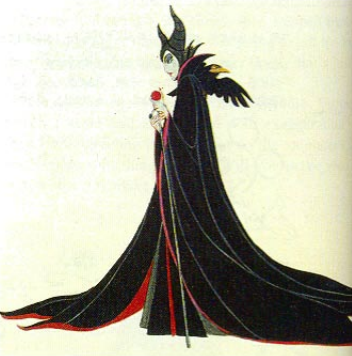
\includegraphics[height=6cm]{Imagenes/sleeping_beauty}
    \caption{Artista: Marc Davis---Sleeping Beauty.}
    \label{fig:sleeping_beauty}
\end{figure}
 
 
 
Un dibujo débil le falta atractivo. Un dibujo que es complicado o difícil de leer le falta atractivo. Un diseño pobre, formas torpes, movimientos raros, 
todas les falta atractivo. A el espectador de gusta ver algo que es atractivo para ellos, ya sea una expresión, un personaje, un movimiento,
o toda una situación histórica. Mientras en actor real tiene carisma, la animación tiene atractivo.\cite{principles_animation}
 
 
\chapter{Animación basada en geometría}
 
 
Estos métodos dependen mucho del animador. 
El movimiento se controla localmente y se define en términos de coordenadas, 
ángulos, velocidades o aceleraciones. El enfoque más simple es el rendimiento de
animación que consiste en la medición magnética u óptica y el registro de acciones 
directas de una persona real para la reproducción inmediata o retrasada. 
La técnica se usa especialmente hoy en entornos de producción para animación de personajes en 3D.
La animación de fotogramas clave \textit{keyframe} es otra técnica popular en la que el animador especifica explícitamente
la cinemática al proporcionar valores de fotogramas clave cuyos fotogramas "intermedios" 
son interpolados por la computadora.\cite{animation_types}
 
 
\section{Animación cuadro por cuadro}
 
La animación de fotogramas claves o cuadro por cuadro \textit{keyframe} en la generación automática de
fotogramas intermedios, llamados inbetweens, basados ​​en un conjunto de \textit{keyframes}
suministrado por el animador. En animación basada en imágenes los \textit{keyframe} o
interpolación de forma, los intermedios se obtienen interpolando el
imágenes de fotogramas clave en sí mismas.\cite{Thalmann}
 
 
En dos dimensiones, la interpolación de formas ha sido popular, especialmente
por el artista Peter Foldes, quién creó maravillosas películas basadas en
esta técnica: \textit{Huger (1974)} y \textit{Metadata (1971).} Esta es un vieja
técnica, introducida por Burtnyk y Wein\cite{burtnyk_wein} Cada \textit{keyframe} son
caracterizados por puntos clave que tienen que corresponder. La figura \ref{fig:interpolation_1} muestra los
principios para crear cuadros intermedios por interpolación lineal entre
puntos correspondientes. Cuando los fotogramas clave correspondientes no tienen el
mismo número de puntos clave, es necesario agregar puntos clave adicionales como
se muestra en la figura \ref{fig:interpolation_2} Un algoritmo de interpolación lineal produce indeseables
efectos como falta de suavidad en el movimiento, discontinuidades en la velocidad
de movimiento y distorsiones en las rotaciones, como se muestra en la figura \ref{fig:interpolation_3}.
 
 
Métodos alternativos han sido propuestos por Baecker\cite{baecker}, Burtnyk y Wein\cite{burtnyk_wein2}, Reeves.\cite{reeves}
Según Steketee y Badler\cite{Steketee_Badler}, no hay un método satisfactorio para la
solución a las desviaciones entre la imagen interpolada y el objeto a modelar.
 
 
Este método puede extenderse a objetos tridimensionales. El principio
es lo mismo cuando los objetos se modelan en marco de alambre. sin embargo, el
La técnica es mucho más compleja cuando los objetos están basados ​​en facetas, porque un
debe encontrarse correspondencia entre facetas y entre vértices.
Se deben agregar vértices y facetas para tener los mismos números para
Ambos objetos. Hong\cite{Hong} ha introducido un algoritmo completo.
 
 
\begin{figure}[ht]
    \centering
    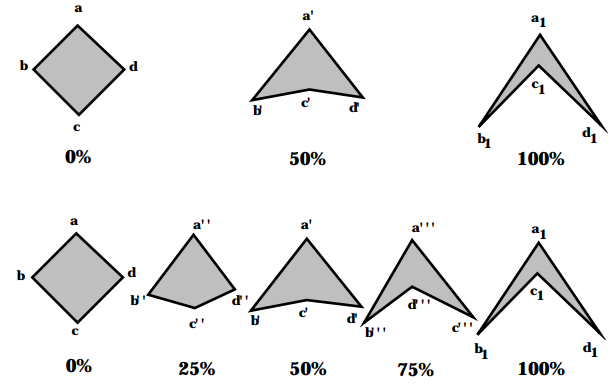
\includegraphics[height=6cm]{Imagenes/interpolation_1}
    \caption{Interpolación lineal}
    \label{fig:interpolation_1}
\end{figure}
 
 
\begin{figure}[ht]
    \centering
    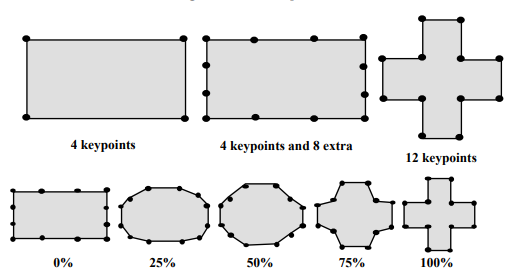
\includegraphics[height=6cm]{Imagenes/interpolation_2}
    \caption{Añadiendo vértices extras antes de la interpolación}
    \label{fig:interpolation_2}
\end{figure}
 
 
\begin{figure}[ht]
    \centering
    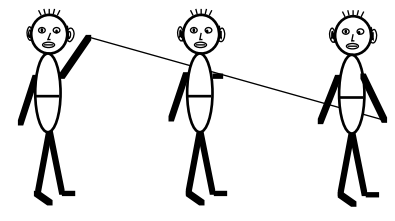
\includegraphics[height=6cm]{Imagenes/interpolation_3}
    \caption{En este ejemplo, la interpolación lineal produce indeseadamente la reducción del brazo}
    \label{fig:interpolation_3}
\end{figure}
 
 
\section{Captura de Movimiento}
 
La captura de movimiento es un proceso popular para generar animación humana.\cite{Bodenheimer}
 
La captura de movimiento tiene sus inicios con los trabajos de Blader\cite{blader1}\cite{blader2} en referencia a la captura y modelado de modelos humanos.
y Bruderlin\cite{bruderlin} en el procesamiento de los datos para la captura de movimiento.
 
 
Si bien la investigación sobre el movimiento humano articulado y la estimación de la pose ha progresado rápidamente en
En los últimos años, no ha habido una evaluación cuantitativa sistemática de métodos competitivos
para establecer el estado actual del arte. Los algoritmos actuales toman muchas decisiones diferentes sobre
cómo modelar el cuerpo humano, cómo explotar la evidencia de la imagen y cómo abordar la inferencia del
problema\cite{state_of_art}
 
 
Los sistemas de captura de movimiento están disponibles comercialmente, y los dos tipos principales de sistemas son ópticos
y magnético En la actualidad, ninguno tiene una clara ventaja sobre el otro, pero los sistemas magnéticos son significativamente más baratos\cite{Bodenheimer}
 
 
\begin{figure}[ht]
    \centering
    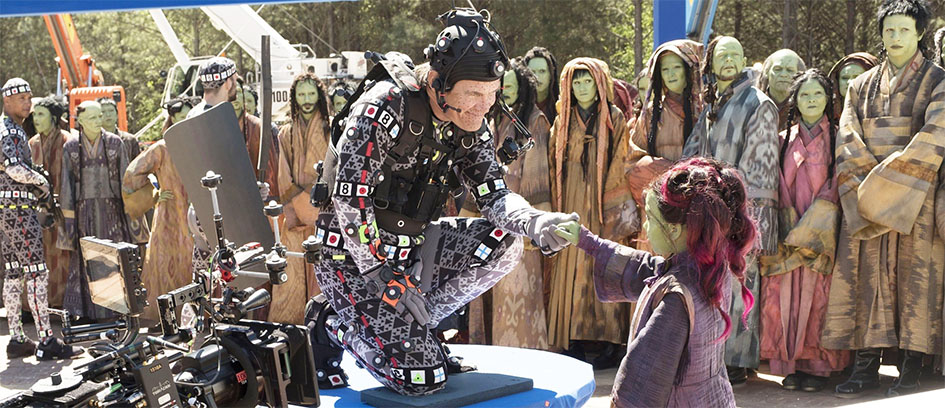
\includegraphics[height=6cm]{Imagenes/motion_capture}
    \caption{Josh Brolin haciendo captura de movimiento \textit{motion capture} en Avengers: Infinity War (Marvel)}
    \label{fig:motion_capture}
\end{figure}
 
 
\chapter{Animación basada en física}
 
 
En estos métodos, el animador proporciona datos físicos y el movimiento se obtiene resolviendo
ecuaciones dinámicas. El movimiento está controlado globalmente. Podemos distinguir métodos basados en
ajuste de parámetros\cite{parametros} y métodos basados en restricciones, donde el animador declara en términos de
limites las propiedades que se supone que tiene el modelo, sin necesidad de ajustar los parámetros.
Por ejemplo, Witkin y Kass\cite{witkin_kass} proponen el concepto de restricciones de espacio-tiempo, para crear
animación de personajes resolviendo las optimizaciones restringidas. Cohen\cite{cohen} lleva este concepto más allá
y usa la ventana de espacio-tiempo para controlar la animación de forma interactiva.
 
\section{Sistema de partículas}
 

Las partículas son los objetos más fáciles de animar. Son objetos que tienen posición, velocidad y masa, pero
sin extensión espacial, es decir, ni momento de inercia ni torque. Las partículas se han utilizado para animar una gran
variedad de comportamientos, como gases, agua, fuego, caucho, ropa, flocado, cuerpos rígidos, etc.\cite{particle_system}
 
Newtonian particles are the most common and are governed by Newton’s second law
 
\begin{equation}
f = m \ddot{r} \Leftrightarrow \ddot{r} = f/m,
\label{eq:1}
\end{equation}
 
 
Donde  \(r(t) \displaystyle = [x_1,x_2,x_3]^T\) es la posición de partida en tiempo t, y
\(\ddot{r} \displaystyle = [\ddot{x_1},\ddot{x_2},\ddot{x_3}]^T = \frac{d^2 r(t)}{dt^2} \) es el
aceleración instantánea de la partícula. La ecuación \(f \displaystyle = m \ddot{r}\) contiene una \textit{derivada de segundo orden},
por lo tanto, es una ecuación diferencial de segundo orden. Las ecuaciones de primer orden son las más simples de resolver, y cualquiera
de las ecuaciones diferenciales lineales de orden superior se pueden convertir a un sistema de diferencial acoplado de ecuaciones de primer orden.\cite{particle_system}
 
 
La animación de fenómenos fluidos es ampliamente utilizada en la industria del cine y tiene una importancia creciente en la
industria de juegos. Navier-Stokes ha descrito con éxito la física de la dinámica de fluidos, con ecuaciones desde aproximadamente 1821,
aunque la investigación posterior sobre fenómenos turbulentos ha agregado considerables
conocimiento sobre el comportamiento de los fluidos a altas velocidades, etc. El modelo Navier-Stokes se usa generalmente para
predecir el movimiento de partículas o volúmenes de fluidos dentro de un fluido completo, pero el modelo también es una buena descripción del
comportamiento de fenómenos gaseosos como el humo a velocidades inferiores a la velocidad del sonido. Para la animación,
la interfaz entre el agua y el aire es igualmente importante, ya que las ondas dominan visualmente las escenas de agua.\cite{particle_system}
 
\begin{figure}[ht]
    \centering
    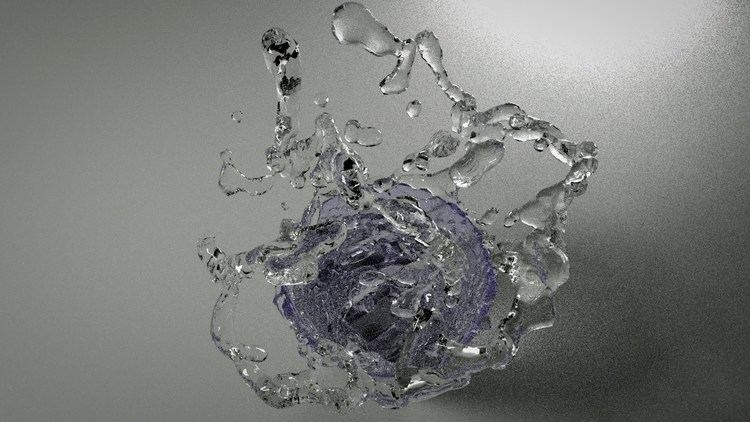
\includegraphics[height=6cm]{Imagenes/fluid_animation}
    \caption{Representacion artistica de animación de fluidos}
    \label{fig:fluid_animation}
\end{figure}
 
 
\chapter{Animación basada en comportamiento}
 
 
Un método de control de movimiento conductual consiste en conducir el comportamiento de criaturas autónomas
proporcionando directivas de alto nivel que indican un comportamiento específico sin ningún otro estímulo.
Reynolds\cite{reynolds} presenta un modelo de comportamiento distribuido para simular bandadas de pájaros y cardúmenes
de pescado Wilhelms\cite{wilhelms}  propone un sistema basado en una red de sensores y efectores. Tu y
Terzopoulos\cite{terzopoulos} describe un mundo habitado por peces artificiales autónomos.
 
 
Uno de los ejemplos tratados en este trabajo fue el de dinámicas agregadas para la simulación de multitudes densas \textit{Aggregate Dynamics for Dense Crowd Simulation}:
 
 
\begin{figure}[ht]
    \hspace*{-2.5cm}
    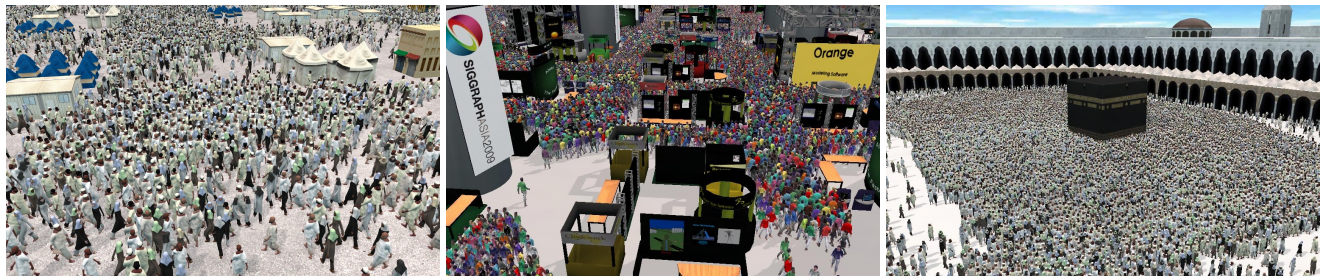
\includegraphics[height=4cm]{Imagenes/agregate_fig}
    \caption{Algunos ejemplos de grandes, densas multitudes simuladas con esta técnica (a) 100,000 peregrinos que se mueven por un campamento
    . (b) 80,000 personas en una convención. (c) 25,000 peregrinos con objetivos heterogéneos en una mezquita.}
    \label{fig:agregate_fig}
\end{figure}
 
 
Las multitudes humanas exhiben un comportamiento altamente complejo impulsado por decisiones individuales de los agentes con respecto a sus objetivos,
obstáculos ambientales y otros agentes cercanos. El problema de simular multitudes virtuales ha atraído cada vez más atención debido a su uso.
para educación y entretenimiento, entrenamiento de emergencia, arquitectura
diseño, planificación urbana, formulación de políticas, ingeniería de tráfico y muchas otras aplicaciones. Los enfoques existentes a menudo simplifican esto
problema separando la planificación global de la prevención local de colisiones. El módulo local para evitar colisiones requiere cada agente
tener en cuenta el movimiento de sus vecinos cercanos; Este paso
se convierte rápidamente en un importante cuello de botella computacional para multitudes muy densas.\cite{agregate}
 
 
Esta observación ha sido explotada por trabajos previos sobre modelos continuos para densidad media de
multitudes [Hughes 2003\cite{Hughes}; Treuille y col. 2006] \cite{Treuille}, y se ha observado
que las multitudes a alta densidad muestran un comportamiento similar a los flujos granulares
[Helbing y col. 2005].\cite{helbing} Esta observación nos motiva a desarrollar un modelo de multitud que describa directamente el movimiento agregado
de la multitud en su conjunto.
 

\chapter{Conclusión}


Si bien la animación es una ilusión, su percepción del mundo real no deja de mantenernos asombrados. Cada vez con animaciones y modelos más realistas, donde vemos
la utilización de \textit{Computer-Generated Imagery} (CGI) en casi todas las películas. Las aplicaciones que tienen crear estos modelos no solo abarca para decir una historia sobre un personaje ficticio,
también puede simular situaciones reales con exactitud. Y no solo en las películas, sino también en juegos y simulaciones médicas y de combate.
 
 
El estado del arte de los modelos de animación ha sido complejo de definir y se han utilizado diferentes métodos para su actualización\cite{state_of_art}
Los modelos de animación hechos a computadora tienen sus inicios a la par cuando las computadoras estaban apenas empezando a mostrar imágenes y
desde ahí solo ha avanzado rápidamente hasta lo que es hoy.
El intento de modelar el mundo real hacia la computadora ha traído nuevas dificultades y también nuevas formas de resolver problemas y se espera que siga avanzando.
 

Se puede llegar a un momento incluso en la inteligencia artificial cuando una computadora puede realmente entender qué es lo que está viendo, no solo como modelos matemáticos, sino como imágenes vivas y animadas.
 
 
 
\begin{thebibliography} {books}
    \bibitem{modelo} Asale, R.-, \& Rae. (n.d.). modelo: Diccionario de la lengua española. Consultado Marzo 15, 2020, en https://dle.rae.es/modelo
    \bibitem{animacion} Animación. (2020, Marzo 12). Consultado Marzo 15, 2020, en https://es.wikipedia.org/wiki/Animación
    \bibitem{sombras_chinescas} Corriente, F. (2014). Consultado Marzo 20, 2020, Del “teatro de sombras” islámico a los títeres, pasando por los ``retablos de maravillas''. Revista de filología española, 94(1), 39-56.
    \bibitem{praxinoscope} Reynaud, E. (2009). Consultado Marzo 20, 2020, Praxinoscope.
    \bibitem{john_whitney} Kirkham, P. (2009). Consultado Marzo 20, 2020, en Vertigo (title sequence), Alfred Hitchcock (1958). Design and culture, 1(2), 218-222.
    \bibitem{sketchpad} Sutherland, I. E. (1964). Consultado Marzo 20, 2020, Sketchpad a man-machine graphical communication system. Simulation, 2(5), R-3.
    \bibitem{animated_hand1} Computer Animated Hand (1972). Consultado Marzo 20, 2020, en https://computeranimationhistory-cgi.jimdofree.com/computer-animated-hand-1972/
    \bibitem{animated_hand2} Holliday, C. (2019). Consultado Marzo 20, 2020, In Good Hands? Indexes and Interfaces in A Computer Animated Hand (Ed Catmull \& Frederic Parke, 1972). In The Crafty Animator (pp. 157-180). Palgrave Macmillan, Cham.
    \bibitem{the_juggler}Adam Powers, The Juggler (1981). (n.d.). Consultado Marzo 20, 2020, en https://computeranimationhistory-cgi.jimdofree.com/adam-powers-the-juggler-1981/
    \bibitem{asas_tron} Reynolds, C. W. (1982). Consultado Marzo 20, 2020, Computer animation with scripts and actors. ACM SIGGRAPH Computer Graphics, 16(3), 289-296.
    \bibitem{IBMR} Debevec, P. (2000, July). Consultado Marzo 20, 2020, Pursuing reality with image-based modeling, rendering, and lighting. In European Workshop on 3D Structure from Multiple Images of Large-Scale Environments (pp. 1-16). Springer, Berlin, Heidelberg.
    \bibitem{immersion} NAIMARK, M., WOODFILL, J., DEBEVEC, P., AND VILLAREAL, L. Immersion ’94. Consultado Marzo 20, 2020, http://www.debevec.org/Immersion/, 1994
    \bibitem{Zabih_Woodfill} ZABIH, R., AND WOODFILL, J. Consultado Marzo 20, 2020, Non-parametric local transforms for computing visual correspondence. In European Conference on Computer Vision (May 1994), pp. 151–158.
    \bibitem{toy_story} Porter, T., \& Susman, G. (2000). Consultado Marzo 20, 2020, On site: Creating lifelike characters in pixar movies. Communications of the ACM, 43(1), 25.
    \bibitem{principles_animation} Johnston, O., \& Thomas, F. (1981). Consultado Marzo 21, 2020, The illusion of life: Disney animation New York: Disney Editions.
    \bibitem{animation_types} Magnenat-Thalmann, N., \& Thalmann, D. (Eds.). (2012). Consultado Marzo 21, 2020, State-of-the-art in Computer Animation: Proceedings of Computer Animation’89. Springer Science \& Business Media.
    \bibitem{Thalmann} Thalmann, N. M., \& Thalmann, D. (1996). Consultado Marzo 21, 2020, Computer animation. ACM Computing Surveys, 28(1), 161-163.
    \bibitem{burtnyk_wein} Burtnyk N, Wein M (1971) Consultado Marzo 21, 2020, Computer-generated Key-frame Animation, Journal SMPTE, 80, pp.149-153.
    \bibitem{baecker} Baecker R (1969) Consultado Marzo 21, 2020, Picture-driven Animation, Proc. AFIPS Spring Joint Comp. Conf., Vol.34, pp.273-288
    \bibitem{burtnyk_wein2} Burtnyk N, Wein M (1976) Consultado Marzo 21, 2020, Interactive Skeleton Techniques for Enhancing Motion Dynamics in Key Frame Animation, Comm. ACM, Vol.19, No10, pp.564-569.
    \bibitem{reeves} Reeves WT (1981) Consultado Marzo 21, 2020, Inbetweening for computer animation utilizing moving point constraints. Proc. SIGGRAPH '81, Computer Graphics, Vol.15, No3, pp.263-269
    \bibitem{Steketee_Badler} Steketee SN, Badler NI (1985) Consultado Marzo 21, 2020, Parametric Keyframe Interpolation Incorporating Kinetic Adjustment and Phrasing Control, Proc. SIGGRAPH '85, pp. 255-262.
    \bibitem{Hong} Hong T.M., R.Laperriere, D.Thalmann, Consultado Marzo 21, 2020, A General Algorithm for 3-D Shape Interpolation in a Facet-Based Representation, Proc. Graphics Interface'88, Edmonton, 1988
    \bibitem{parametros} W.W.Armstrong, M.Green, R.Lake (1987) Consultado Marzo 21, 2020, Near real-time Control of Human Figure Models, IEEE CG\&A, 7( 6)28-38.
    \bibitem{Bodenheimer} Bodenheimer, B., Rose, C., Rosenthal, S., \& Pella, J. (1997). Consultado Marzo 22, 2020, The process of motion capture: Dealing with the data. In Computer Animation and Simulation’97 (pp. 3-18). Springer, Vienna.
    \bibitem{blader1} BADLER, N. I., HOLLICK, M. J., AND GRANIERI, J. P. Consultado Marzo 22, 2020, Real-time control of a virtual human using minimal sensors. Presence 2, 1 (1993), 82–86.
    \bibitem{blader2} BADLER, N. I., PHILLIPS, C. B., AND WEBBER, B. L. Consultado Marzo 22, 2020, Simulating Humans: Computer Graphics Animation and Control. Oxford University Press, Oxford, UK, 1993.
    \bibitem{bruderlin} BRUDERLIN, A., AND WILLIAMS, L. Consultado Marzo 22, 2020, Motion signal processing. In Computer Graphics(Aug. 1995), pp. 97–104. Proceedings of SIGGRAPH 95.
    \bibitem{state_of_art} Sigal, L., \& Black, M. J. (2006). Consultado Marzo 22, 2020, Humaneva: Synchronized video and motion capture dataset for evaluation of articulated human motion. Brown Univertsity TR, 120.
    \bibitem{witkin_kass} A.Witkin, M.Kass (1988) Consultado Marzo 21, 2020, Spacetime Constraints, Proc.SIGGRAPH '88, pp.159-168
    \bibitem{cohen} M.F.Cohen (1992) Marzo 21, 2020, Interactive Spacetime Control for Animation, Proc. Siggraph'92, pp.293-302.
    \bibitem{particle_system}Erleben, K., Sporring, J., Henriksen, K., \& Dohlmann, H. (2005). Consultado Marzo 22, 2020, Physics-based animation (p. 13). Hingham: Charles River Media.
    \bibitem{reynolds} C.Reynolds (1987) Marzo 21, 2020, Flocks, Herds, and Schools: A Distributed Behavioral Model, Proc.SIGGRAPH '87, pp.25-34.
    \bibitem{wilhelms} J.Wilhelms (1990) Marzo 21, 2020, A Notion for Interactive Behavioral Animation Control, IEEE CG\&A, 10(3)14-22
    \bibitem{terzopoulos} X.Tu, D.Terzopoulos (1994) Marzo 21, 2020, Artificial Fishes: Physics, Locomotion, Perception, Behavior, Proc.SIGGRAPH'94, pp.42-48.
    \bibitem{agregate} Narain, R., Golas, A., Curtis, S., \& Lin, M. C. (2009). Consultado Marzo 22, 2020, Aggregate dynamics for dense crowd simulation. In ACM SIGGRAPH Asia 2009 papers (pp. 1-8).
    \bibitem{Hughes} HUGHES, R. L. 2003. Consultado Marzo 22, 2020, The flow of human crowds. Annu. Rev. Fluid Mech. 35, 169–182.
    \bibitem{Treuille} TREUILLE, A., COOPER, S., AND POPOVIC, Z. 2006. Consultado Marzo 22, 2020, Continuum crowds. ACM Trans. Graph. 25, 3, 1160–1168.
    \bibitem{helbing} HELBING, D., BUZNA, L., JOHANSSON, A., AND WERNER, T. 2005. Consultado Marzo 22, 2020, Self-organized pedestrian crowd dynamics: Experiments, simulations, and design solutions. Transportation Sci. 39, 1–24
\end{thebibliography}
 
 
\end{document}
 
 

